\documentclass[tikz, margin=3mm]{standalone}
\usetikzlibrary{arrows.meta,
                chains,
                positioning,
                shapes.geometric
                }
% for fancy looks of data storages
\begin{document}
    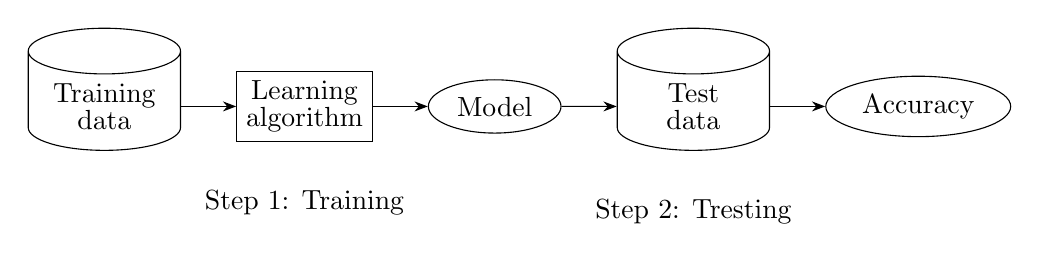
\begin{tikzpicture}[
    node distance = 5mm and 7mm,
    start chain = going right,
    disc/.style = {shape=cylinder, draw, shape aspect=0.3,
                   shape border rotate=90,
                   text width=17mm, align=center, font=\linespread{0.8}\selectfont},
  mdl/.style = {shape=ellipse, aspect=2.2, draw},
  alg/.style = {draw, align=center, font=\linespread{0.8}\selectfont}
                    ]
    \begin{scope}[every node/.append style={on chain, join=by -Stealth}]
\node (n1) [disc] {Training\\ data};
\node (n2) [alg]  {Learning\\ algorithm};
\node (n3) [mdl]  {Model};
\node (n4) [disc] {Test\\ data};
\node (n3) [mdl]  {Accuracy};
    \end{scope}
\node[below=of n2]  {Step 1: Training};
\node[below=of n4]  {Step 2: Tresting};
    \end{tikzpicture}
\end{document}